% !TeX root = ../thesis.tex
\chapter{RekenRangers}
\label{chp:rekenrangers}
The previous chapters identified a gap between classroom exercise tools and controlled research software, and Chapter \ref{chp:problem-statement} formalised that gap as a problem statement. This chapter describes RekenRangers\footnote{Although the application is officially named \textit{RekenRangers}, the English name \textit{MathRangers} may also be used throughout this thesis for readability and convenience.}, the platform built to address it. RekenRangers is a web-based arithmetic learning tool designed for primary school children aged 7 to 11. It is built to function both as a daily classroom exercise tool and as a configurable research instrument, so that the same platform children use to practise arithmetic can also serve as the environment in which researchers run controlled experiments.

The platform is hosted on a KU Leuven server and accessible through any modern web browser at \texttt{https://rekenrangers.cs.kuleuven.be/}, which means it runs on the laptops, tablets\footnote{RekenRangers runs in any tablet browser, but the interface has not been specifically optimised for tablets, and there is currently no tablet application. Both are possible directions for future work.}, and Chromebooks that schools already have without requiring any installation. The back-end is written in Python using the Flask web framework \cite{grinberg2018flask}, with a MySQL database for persistent storage. The front-end uses HTML, CSS, and JavaScript, with the Bootstrap library for responsive layout. The full codebase is maintained in a private GitHub repository.\footnote{The author of this thesis intends to set an open-source license on the repository in the future, so that the platform can be reused, extended, and inspected by other researchers.}

This chapter begins by describing the design process and the decisions that shaped the platform at a high level, then walks through the tool's approach to each of the twelve properties identified in Chapters \ref{chp:background} and \ref{chp:exercise-tools}.

\section{Design process and guiding principles}
RekenRangers was not designed in isolation. Building a tool that needs to work for children, teachers, and researchers at the same time is hard to do without input from all three groups, and the design process was set up to make at least some of that input possible. While the project did not involve frequent direct meetings with teachers or children, advice was sought from these groups at key moments, and the design was continuously discussed with the researchers who would eventually use the tool in their own studies. Research in educational technology has consistently shown that involving stakeholders early and continuously in the design process leads to tools that are more likely to be adopted and that better fit the needs of the people who will actually use them \cite{cumbo2022participatory}.

The core development, both back-end and front-end, was carried out by the author of this thesis. Design decisions, however, were shaped through continuous collaboration with several key partners. Throughout the project, the author's supervisor, Prof. Dr. Tom Schrijvers, provided guidance on the overall direction of the work and feedback on its development. On the educational-research side, the co-supervisor of this thesis, Elien Bellon, contributed both the scientific grounding for the platform's features and a concrete benchmark study to replicate, drawing on her own research on metacognitive monitoring in arithmetic \cite{bellon_more_2019, bellon2020, bellon2021}. Two master's students in pedagogical sciences at KU Leuven, Eline T'joen and Kiara Willems, were also closely involved, since their own theses depended on using RekenRangers in classroom settings. Their involvement meant that design decisions were tested against real use cases from the start: if a feature did not make sense to someone planning a study with third-graders, it was reworked. A final, less direct source of input was the set of existing tools discussed in Chapters \ref{chp:background} and \ref{chp:exercise-tools}. These tools served a dual role. Rekentuin and Automatus provided models for what a child-friendly arithmetic tool looks and feels like, from adaptive difficulty to avatar systems to coin-based reward structures. OpenSesame and PsychoPy provided a clear reference for the kinds of experimental control and data logging a research tool must offer, but they also provided a vivid image of what happens when engagement is not a priority. The black-screen, stimulus-response experience that characterises most experiments built in these tools (see Figure~\ref{fig:black_screen}) was a constant reminder of what RekenRangers needed to avoid.

This combination of perspectives shaped two core principles that guided the design throughout.

The first was that the replication of the Bellon et al. study \cite{bellon_more_2019} had to be possible. This study, which investigates the relationship between metacognitive monitoring and arithmetic performance in children, lived in the back of the author's mind throughout development: it was a concrete example of a study that had already been run in OpenSesame and that the researchers involved had found difficult to set up there. It was not used as a checklist that every feature was tested against, but it acted as a recurring reference point that kept the development grounded in a real research need rather than in abstract feature lists.

The second was a matter of audience. RekenRangers needed to be configurable by people who do not write code and feel like a game to the children using it. These are essentially restatements of the central goals identified in Chapters \ref{chp:background} and \ref{chp:exercise-tools}, but they were treated as design principles in their own right: every screen, every flow, and every configuration option was evaluated against whether it served a non-programming researcher on one side and a seven-year-old on the other.

Generative AI tools were used during development to assist with specific implementation tasks such as generating boilerplate code and debugging. All architectural decisions, feature design, and user interface design were made by the author in collaboration with the partners described above.

The following section describes how each of the twelve properties from Chapters \ref{chp:background} and \ref{chp:exercise-tools} was addressed in the design and implementation of RekenRangers.

\section{Approach: design decisions per property}
This section walks through each of the twelve properties from Chapters \ref{chp:background} and \ref{chp:exercise-tools} and describes how RekenRangers addresses them. The research-tool properties are discussed first, followed by the exercise-tool properties.

\subsection{Data tracking}
\label{sec:data-tracking}
Section \ref{sec:research-properties} defined data tracking as the most basic requirement of any research tool: the tool must record what happens, completely and automatically. In RekenRangers, every exercise completed by every child produces a full data record that is stored in the database. The level of detail was determined in close collaboration with Eline T'joen, Kiara Willems, and co-supervisor Elien Bellon, to ensure that the logged data would be sufficient for the kinds of analyses that arithmetic research requires.

Each record captures the full context of a single exercise: who answered, the operation and operands presented, the answer given, whether it was correct, and the response time. The record also includes the difficulty level, whether the timer was visible, the child's current Elo rating and the change in rating produced by that exercise, and the difficulty zone the child was in at the time. When the metacognitive self-assessment is enabled, the confidence judgement is logged together with a calibration field capturing whether the self-assessment matched the actual outcome. Response times are recorded separately for the exercise, the confidence judgement, and the feedback screen, which lets researchers analyse not just what children answered but how long they spent on each phase of the trial. The complete list of fields is given in Appendix~\ref{app:data-fields}.

This data is accessible in two ways. The teacher dashboard, when a student is selected from the group overview, shows the full list of exercises that student has completed, at a level of detail aimed at the teacher rather than at the researcher. For research purposes, the group screen offers an export function that generates a single CSV file containing every exercise completed by every student in the group. This file can be opened directly in Excel or imported into statistical software for analysis. The export is designed to require no preprocessing: each row is one exercise, each column is one variable, and no manual cleaning or restructuring is needed before the data can be used.

\subsection{Experimental control}
\label{sec:experimental-control}
Experimental control is the property that most clearly separates a research tool from a classroom tool. Section \ref{sec:research-properties} defined it as the ability to dictate precisely what each participant sees and under what conditions, so that the researcher can isolate the variables they are studying. In RekenRangers, experimental control is implemented through a layered settings system in the teacher dashboard, where each group of children can be configured independently.

The first layer covers the general exercise settings. For any group, the teacher or researcher can choose which arithmetic operations are available, how difficulty is determined (adaptive, fixed, or chosen by the child), whether a timer is shown, and whether metacognitive self-assessment prompts are enabled. These settings are sufficient for classroom use and for simple studies where the main concern is controlling what type of exercises children see. The full list of configurable settings is provided in Appendix~\ref{app:group-settings}.

The second layer covers the research settings (Figure~\ref{fig:research-settings}), where the experimental control becomes precise. The most important option here is \textit{research mode}. When research mode is enabled, the interface changes in ways that are invisible to the child but critical for the researcher. Mouse interaction is disabled entirely, so that all input happens through the keyboard. Buttons and interface elements that are not essential to the exercise flow are hidden or deactivated, reducing the chance that a child accidentally navigates away from the task or gets distracted by something outside the experiment. Several pieces of interface text are also adjusted: in normal mode some labels offer the child additional options that are no longer available in research mode, so the corresponding text is replaced with a research-mode equivalent. In short, research mode strips the interface down to what the experiment requires and nothing more.

Within the research settings, a set of item generation rules gives the researcher fine-grained control over which exercises can appear. Identical exercises can be blocked from appearing twice within the same session. Tie problems, where both operands are the same number (such as \(4+4\) or \(7 \times 7\)), can be excluded because they are known to be solved through different processes than non-tie problems \cite{campbell2002tie}. Exercises that produce the same result can be prevented from appearing consecutively. Commutativity can be enforced, so that \(3 \times 7\) and \(7 \times 3\) are registered as the same exercise. The position of the larger operand can be balanced across trials to prevent children from developing a position bias. Beyond these structural rules, the researcher can define exclusion lists for specific operand values and results, for example excluding 0, 1, or 11. A fixation screen can also be enabled before each exercise, which is standard practice in reaction-time research to ensure the child is focused before the stimulus appears.

Effort also went into ensuring that children cannot inadvertently break the experimental flow. In research mode, there is no way to skip an exercise, navigate to the puzzle screen mid-session, or exit the exercise sequence (except through browser actions). Answers are constrained to valid numerical input, and the interface enforces a fixed progression from exercise to self-assessment to feedback to the next exercise. In a classroom with twenty children working simultaneously and no researcher behind each screen, these details are the difference between clean data and a session that has to be discarded.

The combination of the general settings and the research-specific controls means that a researcher can configure two groups within the same classroom to see identical exercises but with different feedback conditions, or the same feedback conditions but with different difficulty settings, without writing any code.

\begin{figure}
\centering
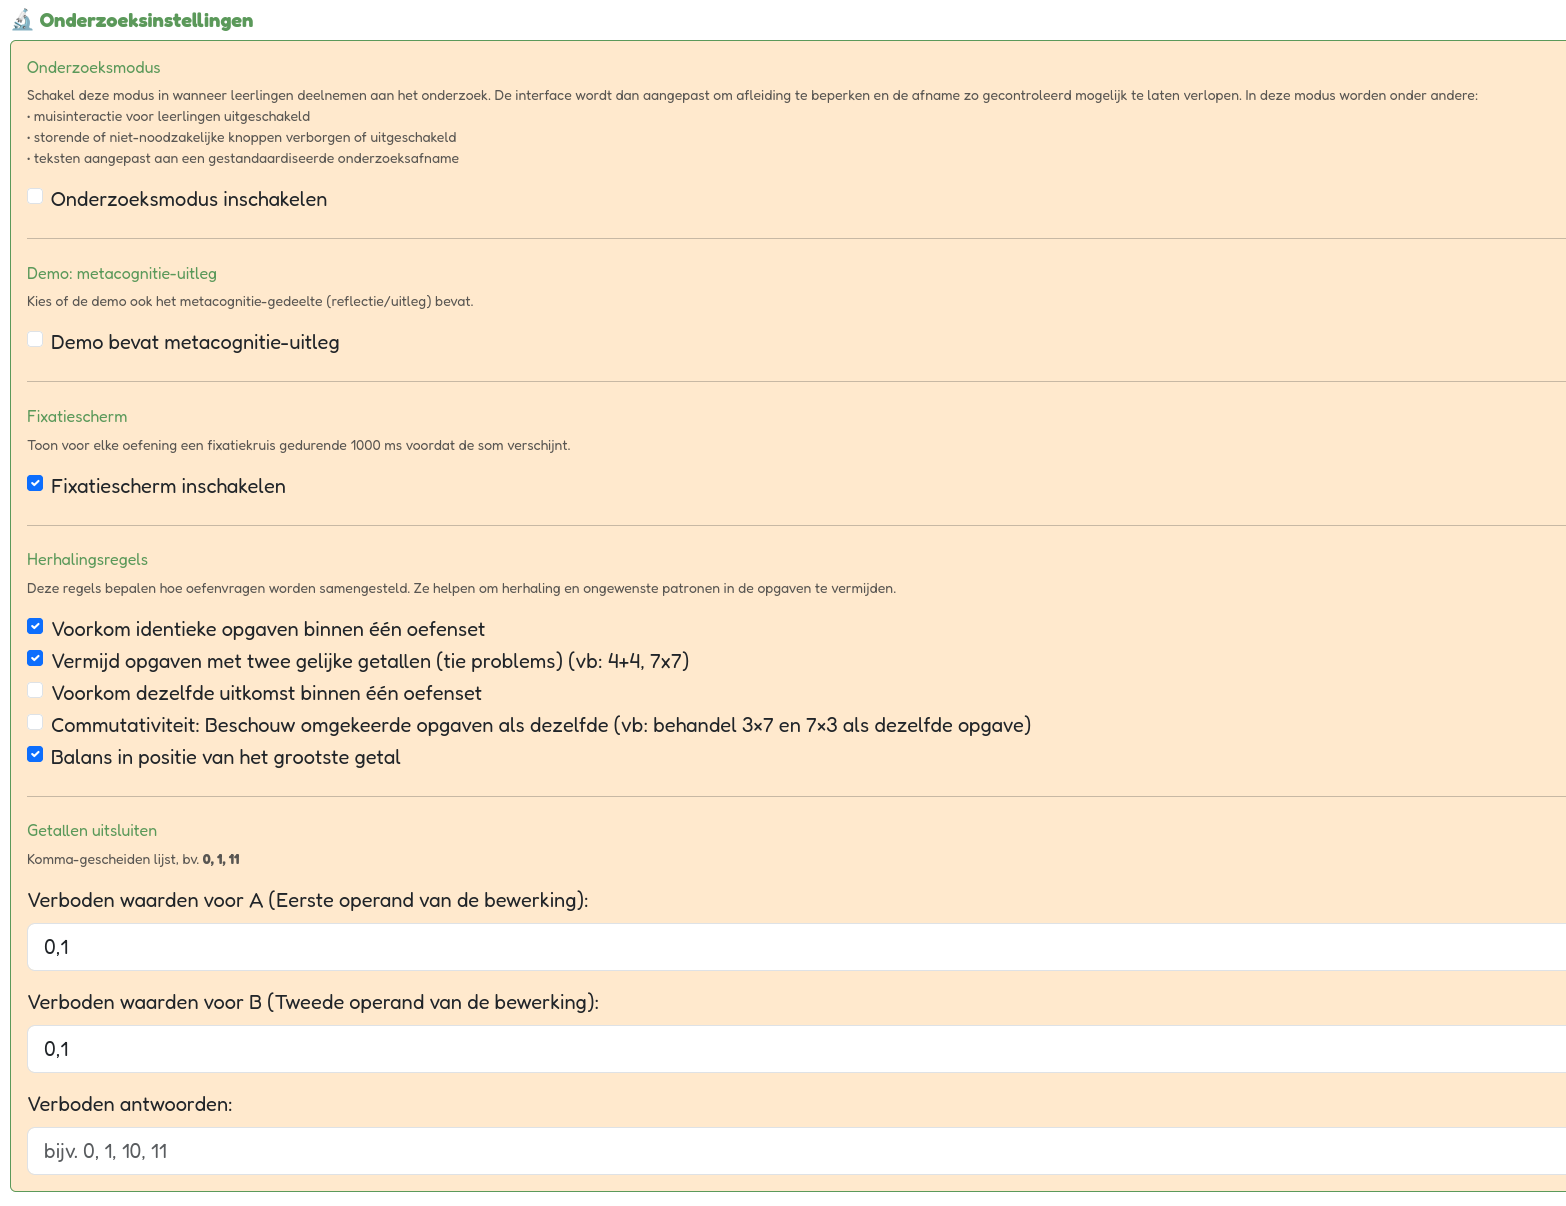
\includegraphics[width=0.85\textwidth]{figures/research-settings-new.png}
\caption{Research settings panel. Researchers can enable research mode, configure item generation rules (e.g.\ tie-problem exclusion, commutativity), define operand exclusion lists, and enable a fixation screen.}
\label{fig:research-settings}
\end{figure}

\subsection{Reproducibility}
Section \ref{sec:research-properties} defined reproducibility as the ability to save, share, and rerun the exact configuration of an experiment. RekenRangers supports this through a JSON-based export and import system, an idea suggested by Tijs Bellefroid. Every setting described in the previous section, from the operation selection to the research-mode rules to the exclusion lists, can be exported to a single JSON file with one click. A second researcher who wants to replicate the study can import that file into their own group, and every setting is restored exactly as it was. Sharing an experimental setup is then as simple as sharing a file.

One important consideration: two children configured with the same settings will not necessarily see the same sequence of exercises. The settings constrain which exercises are allowed, but the choice of which specific exercise comes next is partly random within those constraints. This is reproducibility at the level of experimental conditions, not at the level of literal trial-by-trial identity, which is the level that matters for between-group comparisons.

\subsection{Flexibility}
\label{sec:flexibility}
Flexibility, as defined in Section \ref{sec:research-properties}, is about whether a tool can support a wide variety of experimental designs without requiring the researcher to modify the underlying code. The settings system described in the previous sections already contributes to this: the ability to configure operations, difficulty modes, metacognitive prompts, timer settings, and item generation rules means that a single installation of RekenRangers can host studies with very different designs. But settings alone are not enough. Most research designs in educational psychology do not consist of a single uniform block of exercises. They involve phases: a warm-up, a main task, a break, a post-test, sometimes with different conditions across phases.

RekenRangers addresses this through an exercise sequence system. A sequence consists of multiple blocks, each with its own settings for the number of exercises, the operation, the difficulty mode, and whether metacognitive prompts are enabled. A researcher can, for example, configure a sequence that starts with 10 easy addition exercises as a warm-up without self-assessment, followed by three blocks of 15 adaptive exercises with metacognitive prompts, and a final block of 10 fixed-difficulty exercises as a post-test. Each block is independently configurable, and blocks can be added, edited, reordered, or removed through the dashboard. The research settings (research mode, exclusion rules, fixation screen) apply to the entire sequence rather than per block, which ensures consistency across phases.

The teacher dashboard also provides tools for managing progress through a sequence. The progress of individual students or the entire group can be reset to the beginning of the first block, which is useful when a session needs to be restarted or when the same sequence is used across multiple days. On the student side, a visual progress indicator shows the child where they are in the sequence, and how many blocks remain before they can puzzle. Figure~\ref{fig:sequence-screen} shows the sequence configuration screen in the teacher dashboard.

\begin{figure}
\centering
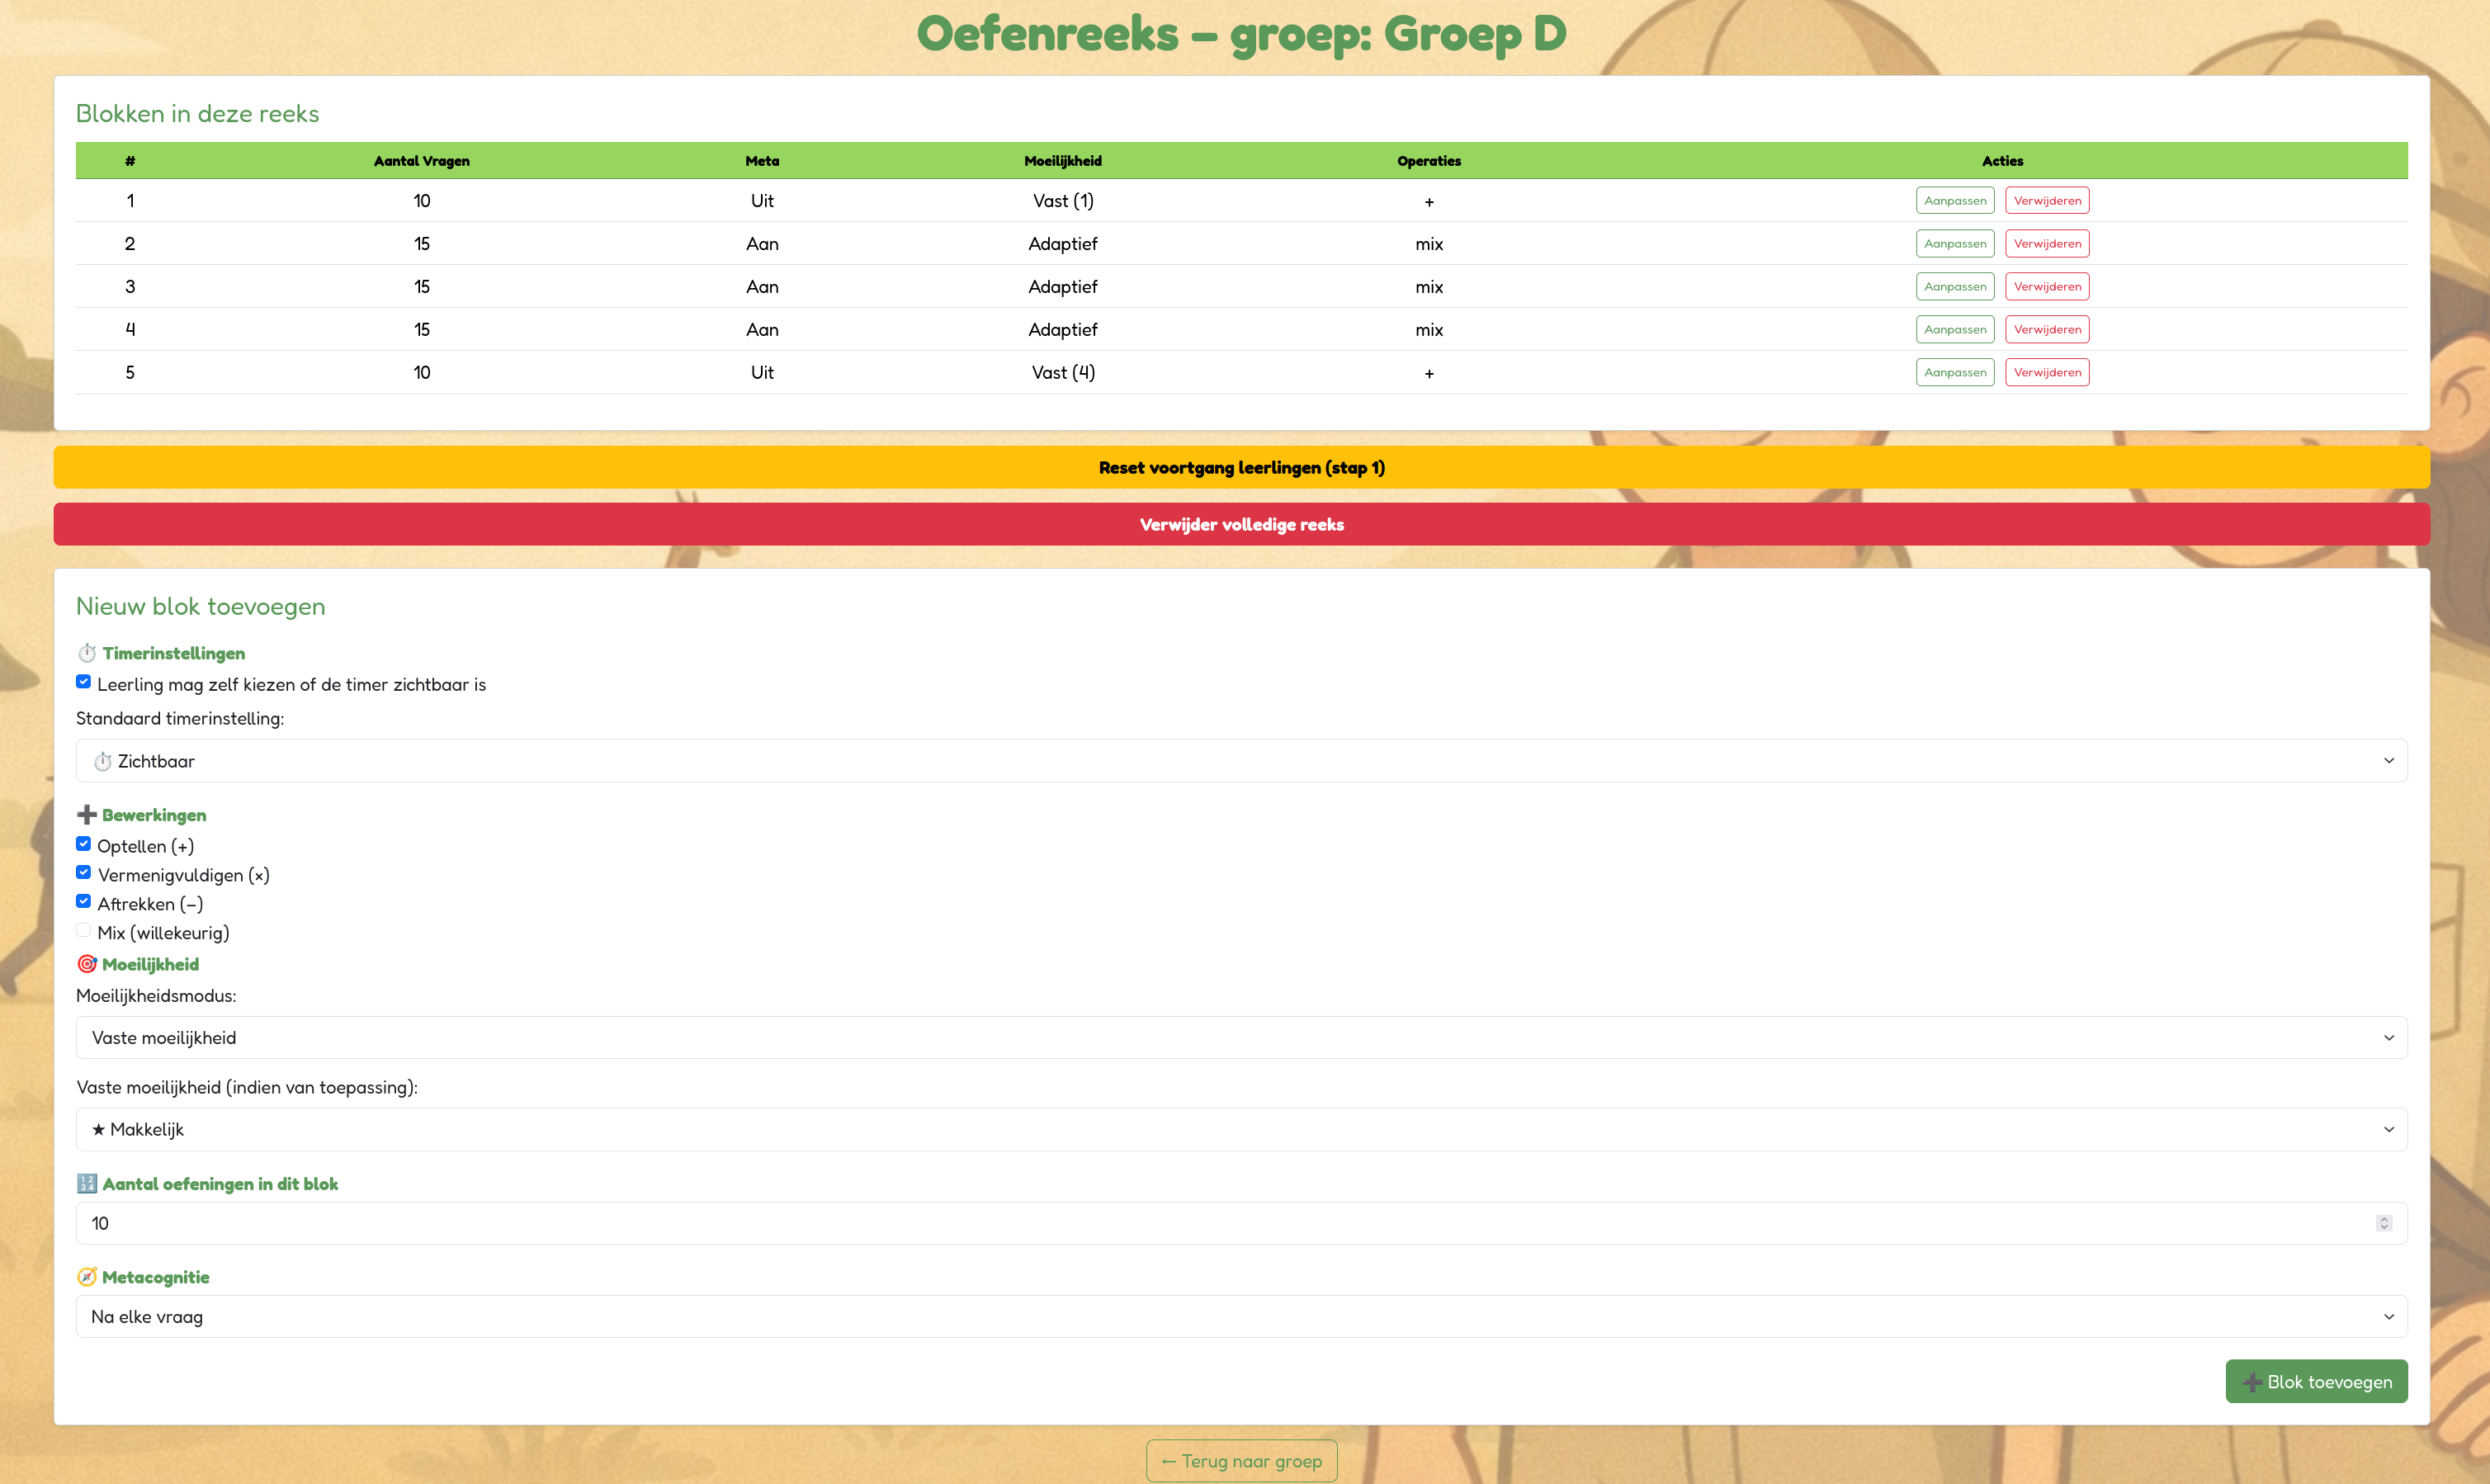
\includegraphics[width=0.8\textwidth]{figures/sequence-screen-new.png}
\caption{The exercise sequence configuration screen. Each row represents a block with its own settings. Blocks can be added, edited, or removed, and student progress can be reset individually or for the entire group.}
\label{fig:sequence-screen}
\end{figure}

The sequence system tries to make RekenRangers more flexible than any of the exercise tools discussed in Chapter \ref{chp:exercise-tools}, and for the kinds of studies it was designed to support, the configurability is sufficient. It does not, however, match the flexibility of a general-purpose programming environment: studies that require trial structures outside the block model, custom adaptive algorithms, or stimulus types beyond arithmetic cannot be expressed within the current tool. This reflects what Lidwell, Holden, and Butler call the ``flexibility--usability tradeoff'': ``as the flexibility of a system increases, the usability of the system decreases'' \cite{lidwell2010universal}. The limits it imposes on RekenRangers are discussed further in Section \ref{sec:limitations}.

\subsection{Reliability}
Section \ref{sec:research-properties} described reliability as having two dimensions: the tool must be robust, stable, and precise in its measurements, and it must keep running under real-world conditions on the kind of hardware schools actually have. RekenRangers addresses both.

On the robustness side, the platform is hosted on a KU Leuven server running inside a containerised environment using Podman and Docker, which isolates the application from the underlying system and makes deployment reproducible and stable. The MySQL database ensures that all data is persistently stored the moment an exercise is completed. If a child's browser crashes mid-session, or if the school's internet drops briefly, the data from every exercise completed up to that point is safe and does not need to be re-collected. The child can log back in and continue from where they left off without losing progress.

On the measurement side, response times are handled in JavaScript on the child's local machine. The timer for an exercise starts when the browser has fully rendered the stimulus on screen, and stops when the child submits their answer. This means that response times reflect actual thinking time rather than being inflated by network latency or server processing delays. The same local timing approach is used for the self-assessment and feedback phases.

The platform was tested across a range of common browsers and some small pilot sessions during development. A more substantial test of how RekenRangers holds up under real classroom conditions is provided by the experiment described in Chapters \ref{chp:experimental-setup} and \ref{chp:results}, with its outcomes discussed in Chapter \ref{chp:discussion}. It is worth noting up front, however, that RekenRangers has not been benchmarked against the kind of formal millisecond-level timing study that has been carried out for tools like PsychoPy \cite{bridges2020timing}.

\subsection{Ease of setup}
The design principle that no feature should require programming knowledge runs through the entire teacher and researcher experience. Every setting discussed in the previous sections, from operation selection to research mode configuration to exercise sequence design, is controlled through dropdown menus, checkboxes, toggle switches, and input fields in a graphical dashboard. There are no configuration files to edit, no scripts to write, and no command-line tools to learn. A researcher who wants to set up a study with three blocks of adaptive multiplication exercises with metacognitive prompts and tie-problem exclusion can do so in a few minutes without ever leaving the browser.

The exercise sequence system in particular benefits from its visual presentation. Each block in a sequence is displayed as a row in a table showing its key settings at a glance, which makes it easy to verify that the experimental design matches the intended protocol. Blocks can be added, reordered, or removed with a single click, and changes are saved immediately. This kind of visual configuration is one of the clearer differences with the research tools discussed in Chapter \ref{chp:background}, where similar functionality would typically require writing and maintaining a Python script.

The teacher and researcher dashboard was designed to be self-explanatory, but for users who need additional guidance a comprehensive manual has been developed that explains every feature and setting in detail. The manual was drafted with the help of generative AI to speed up the writing, and then checked manually to make sure every described feature behaves as written. It is available both within the platform itself\footnote{\url{https://rekenrangers.cs.kuleuven.be/static/handleiding_leerkracht.html}} and as a standalone document included in Appendix~\ref{app:teacher-manual}. A video walkthrough is also available.\footnote{\url{https://youtu.be/jeK2u8FNoPU}}

There is also room for improvement on this front, for example a preview of what the child will see given the current configuration, or a visual timeline of the exercise sequence rather than a table. The current setup interface is functional but does not yet scale with the number of options it now supports, which is one of the limitations of the platform discussed further in Section \ref{sec:limitations}.

\subsection{Adaptivity}
\label{sec:adaptivity}
A core requirement identified in Section \ref{sec:exercise-properties} is that exercises should match the child's current ability level. RekenRangers implements this through an adaptive difficulty system inspired by the Elo rating principle, informed by the work of Klinkenberg et al. on the adaptive engine behind Rekentuin \cite{klinkenberg2011computer}. The system described below was developed in collaboration with Eline T'joen and Kiara Willems.

The central idea is that each child maintains a numerical rating that reflects their estimated skill level. This rating starts at 450 on a scale from 0 to 1000 and is updated after every exercise using the standard Elo update rule:

\begin{equation}
\theta'_j = \theta_j + K(S{ij} - E(S_{ij}))
\end{equation}

where \(\theta_j\) is the child's current rating, \(S_{ij}\) is the score obtained on the exercise, and \(E(S_{ij})\) is the expected score. The paramter \(K\) controls how strongly the rating reacts to each answer and was set to \(K = 20\) after callibration across two pilot studies in the classroom settings.\footnote{In the current version of RekenRangers, \(K\) is fixed at 20. Making this a configurable setting in the teacher dashboard is a natural next step.}

The expected score is fixed at \(E(S_{ij}) = 0.75\). This value was chosen based on findings in the adaptive learning literature suggesting that a target success rate around 75\% keeps learners in a productive zone: high enough to maintain confidence, but low enough that the task remains challenging \cite{klinkenberg2011computer}. The system converges toward a state where the child answers roughly three out of four exercises correctly.

How the actual score \(S_{ij}\) is computed depends on whether the child answered correctly. An incorrect answer always results in \(S_{ij} = 0\), which produces a rating decrease. A correct answer incorporates response time through a quadratic scoring function:

\begin{equation}
\label{for:scoring-function}
S_{ij} = -\frac{5}{4d_i^2} \cdot t_{ij}^2 + 2
\end{equation}

where \(t_{ij}\) is the time the child took and \(d_i\) is the time limit for that exercise (15, 20, or 25 seconds for easy, medium, and difficult exercises respectively). This function has a natural interpretation. If the child answers exactly at the time limit, the score equals 0.75, which matches the expected score and produces no rating change. Answering faster yields a score above 0.75 and pushes the rating up. This means the system does not just track whether a child can solve a problem, but also how fluently they can solve it.

The rating then determines which exercises the child sees. Exercises are categorised into three difficulty levels (easy, medium, and difficult), and the system selects from a probability distribution that shifts with the rating, as shown in Table~\ref{tab:difficulty-zones}. A child below a rating of 250 receives mostly easy exercises, between 250 and 800 a mix dominated by medium exercises, and above 800 mostly difficult ones. Since children start at a rating of 450, they begin in the middle zone with a mix of all three levels. As they improve, the distribution shifts toward harder problems; if they struggle, it shifts back. The system is self-correcting and adjusts to each child individually, without the teacher needing to intervene.

What counts as easy, medium, or difficult depends on the operation and involves constraints on the operands (see Section~\ref{sec:experimental-control}), the result, and whether carrying or borrowing is required. The progression follows the same logic across operations: easy exercises stay within single-digit arithmetic, medium exercises introduce two-digit numbers without carrying or borrowing, and difficult exercises add that step. The full specification is provided in Appendix~\ref{app:exercise-spec}.

\begin{table}
\centering
\begin{tabular}{lll}
\toprule
Difficulty zone & Rating range & Exercise distribution \\
\midrule
1 & 0 -- 200 & 100\% easy \\
2 & 200 -- 400 & 70\% easy, 30\% medium \\
3 & 400 -- 600 & 70\% medium, 20\% easy, 10\% difficult \\
4 & 600 -- 800 & 70\% difficult, 30\% medium \\
5 & 800 -- 1000 & 100\% difficult \\
\bottomrule
\end{tabular}
\caption{Difficulty zone distribution based on participant rating. Children are gradually exposed to harder exercises as their estimated ability increases.}
\label{tab:difficulty-zones}
\end{table}

It is worth noting that adaptivity in RekenRangers is configurable rather than fixed. In research mode, the teacher or researcher can disable the adaptive system and fix the difficulty at a specific level, which is essential for studies that require identical conditions across participants. This and the other research-control settings are discussed in Section~\ref{sec:experimental-control}.

\subsection{Engagement}
Section \ref{sec:exercise-properties} identified engagement as the property that determines whether children actually want to use a tool, not just whether they can. For RekenRangers, this meant that simply presenting arithmetic exercises in a clean interface was not enough. The tool needed a reason for children to care, a narrative that gave the exercises meaning beyond getting the right answer.

The narrative developed for RekenRangers is built around a safari theme. The children are rangers (hence the name RekenRangers) and their mission is to rescue animals that have been captured by poachers. Solving arithmetic exercises earns coins, and coins are spent on puzzle pieces that gradually reveal an image of the animal. Once a puzzle is complete, the animal is freed. This framing turns every exercise session into a small step toward a visible goal, which gives even a routine practice session a sense of purpose.

The coin system is tied directly to performance. Children earn more coins for correct answers and for answering quickly, which creates a natural incentive to stay focused without the competitive pressure of leaderboards or peer comparison. The puzzles add a second layer of motivation: animals cost different amounts to rescue, so children have to choose which animal to work on next, and completing a more expensive puzzle feels like a bigger achievement. Figure~\ref{fig:puzzle-home} shows the puzzle selection screen.

\begin{figure}
\centering
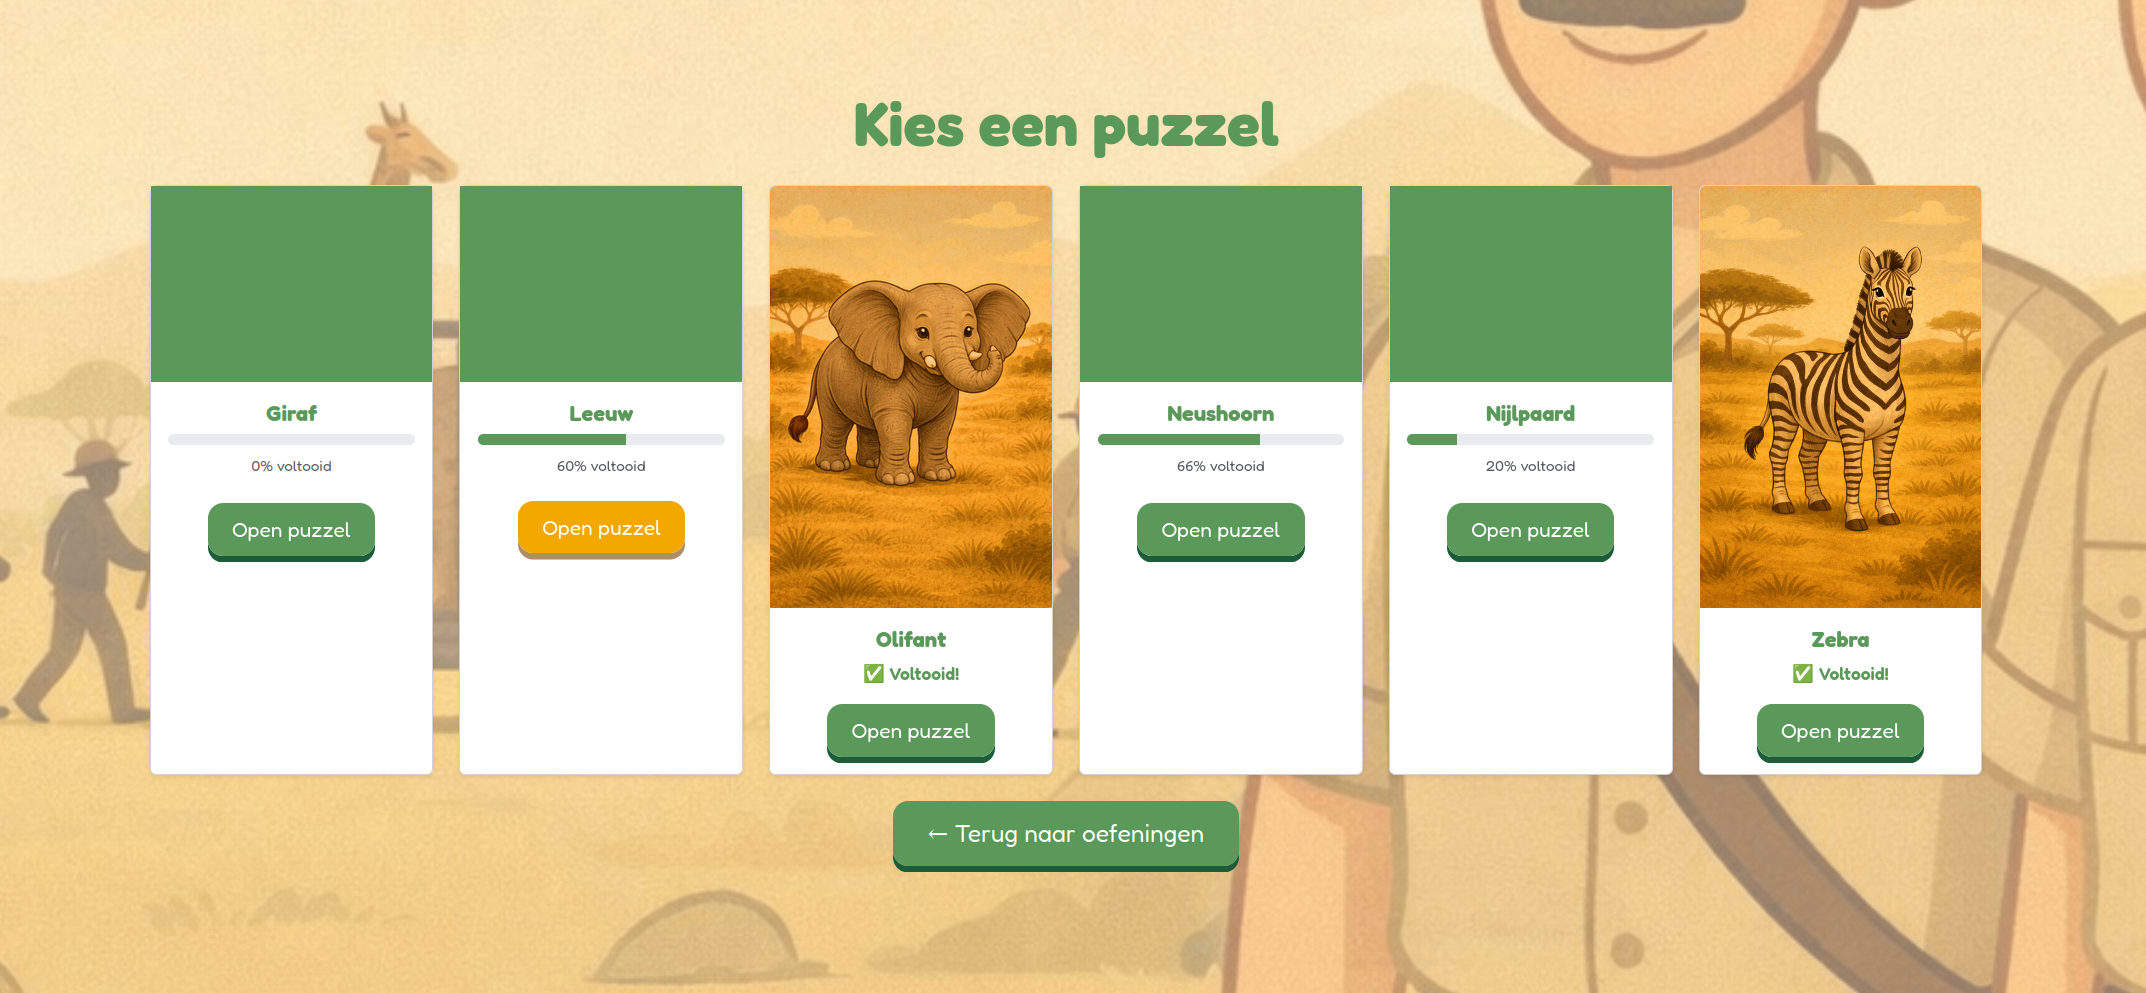
\includegraphics[width=0.85\textwidth]{figures/puzzle-home-new.png}
\caption{The RekenRangers puzzle environment. }
\label{fig:puzzle-home}
\end{figure}

The safari theme is not limited to the reward system. It runs through the entire application: the background illustrations, the button styles, the icons, and the login screen are all designed around the same visual identity. This consistency reinforces the idea that the child is inside a world, not just using a tool. All visual assets, including background scenes and animal images, were created using generative AI and then selected and adapted to fit the visual style of the application.

\subsection{Feedback}
After every exercise, the child receives immediate feedback on their answer. If the answer is correct, the screen shows a short confirmation message. If the answer is wrong, the correct answer is displayed alongside the child's attempt, so that the child can see exactly where they went wrong. The feedback is deliberately kept simple and direct: no elaborate explanations or worked-out solutions, just a clear signal of correctness and, when needed, the right answer. This choice connects back to Section~\ref{sec:exercise-properties}, where the literature on educational feedback suggested that minimal, focused feedback can support children's persistence and strategy use at least as well as more elaborate variants. Extending this with worked-out explanations or hints could still be valuable, particularly for harder operations, and was kept simple here partly because the scope of the supported exercises (single-step addition, subtraction, and multiplication) and the time constraints of the project did not require more.

When the metacognitive self-assessment setting is enabled, a second layer of feedback is added. After each exercise, the child is asked to judge their own answer using a row of four smileys ranging from confident-correct (green) to confident-wrong (red). Once both the answer and the self-assessment are submitted, the feedback screen evaluates both. The self-assessment is considered correct if the child's confidence matched the actual outcome: selecting green or yellow when the answer was right, or orange or red when it was wrong. If the child misjudged their own performance, the feedback tells them so explicitly. Figure~\ref{fig:feedback-screen} shows an example of an exercise that was answered incorrectly but where the child correctly anticipated the mistake.

\begin{figure}
\centering
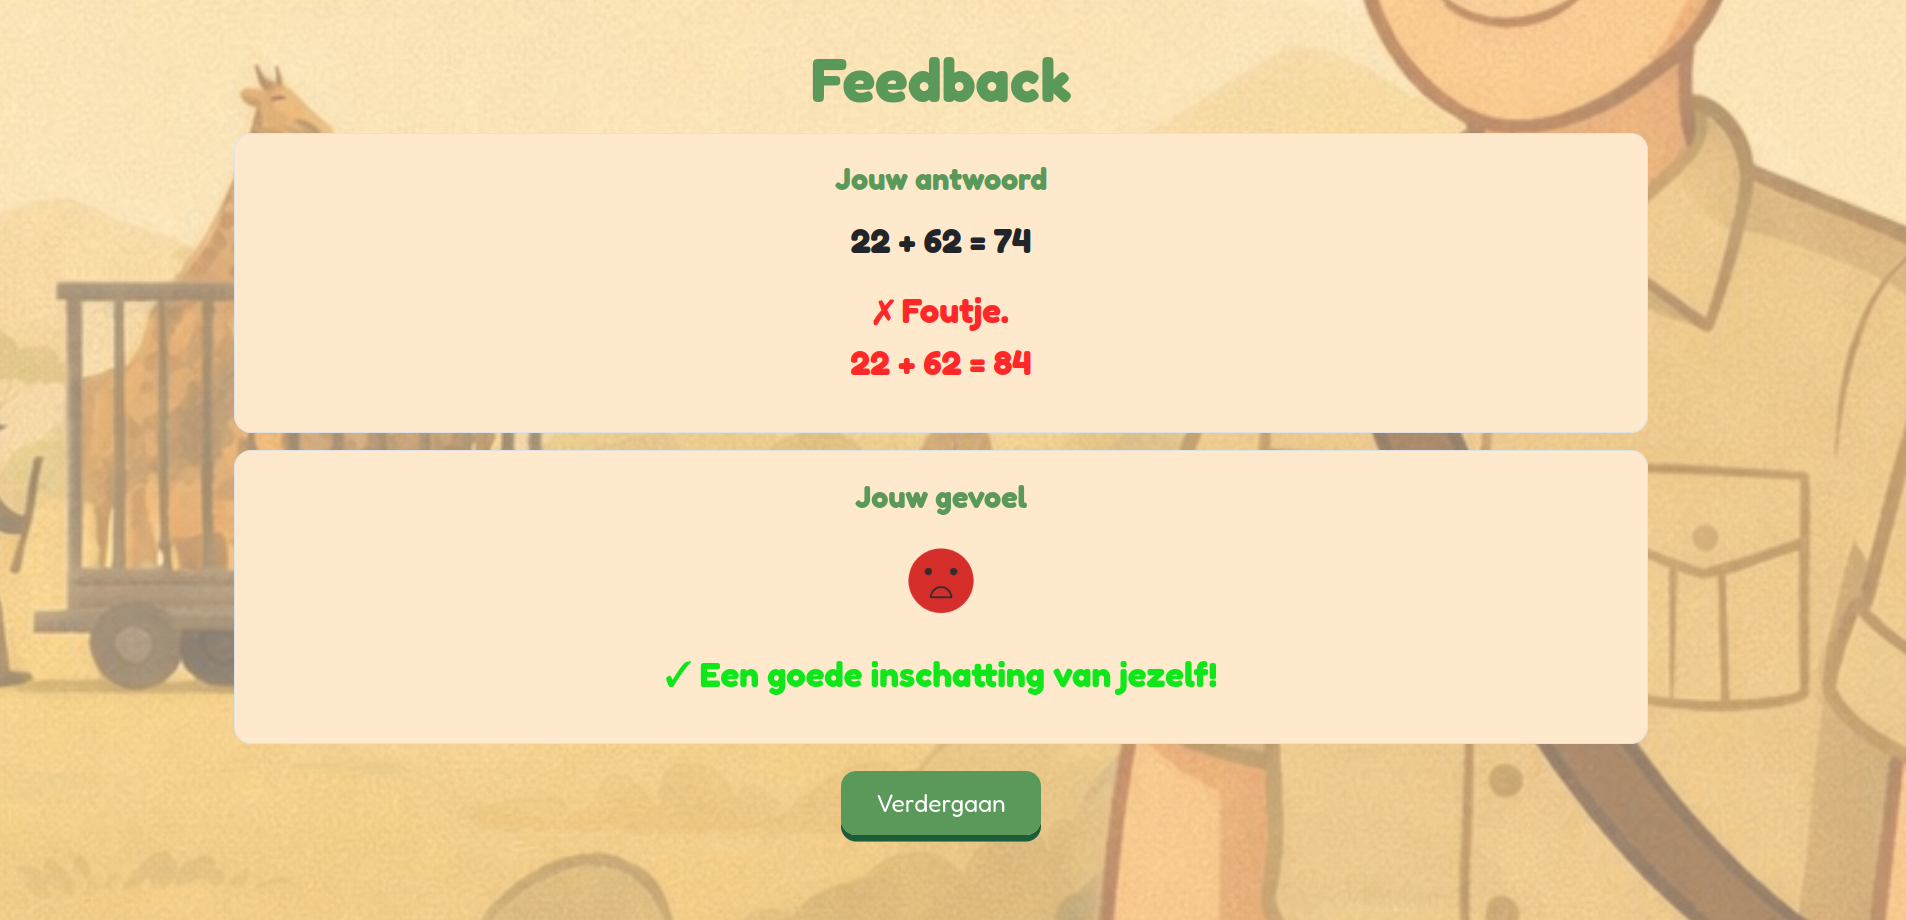
\includegraphics[width=0.85\textwidth]{figures/feedback.png}
\caption{Feedback screen after an incorrectly answered exercise, where the child correctly anticipated the mistake through their self-assessment.}
\label{fig:feedback-screen}
\end{figure}

The confidence judgement paradigm used here mirrors the one in the Bellon et al. study \cite{bellon_more_2019}, and the smileys give it a visual language that is accessible to children as young as seven.

\subsection{Personalisation}
Personalisation is the property where RekenRangers has the most room for growth. The original intention was to integrate an avatar system into the safari theme, where each child would have their own ranger character that could be customised with outfits and accessories purchased with earned coins. Due to time constraints and the need to prioritise the research-critical features, this was not implemented in the current version of the platform.

What RekenRangers does offer is a form of functional personalisation. When enabled by the teacher or researcher, children can choose for themselves which operation they want to practise, what difficulty level they prefer, and whether they want to see a timer. These choices give children a degree of control over their own learning experience, which as discussed in Section \ref{sec:exercise-properties} can support metacognitive awareness and a sense of ownership. Additionally, each child works with their own account, and their coin balance and puzzle progress are personal to them. A child who has saved up coins and completed three animal puzzles sees a different puzzle screen than a classmate who just started. This creates some sense of individual identity within the platform, even without a visual avatar.

The foundation for deeper personalisation is in place. The account system, the coin economy, and the safari theme all lend themselves naturally to extensions such as customisable ranger avatars, personal statistics dashboards, or achievement badges. These are realistic additions for future development and would strengthen a property that is currently functional but not yet fully realised.

\subsection{Accessibility}
RekenRangers is a web application hosted on a KU Leuven server and accessible at \texttt{rekenrangers.cs.kuleuven.be}. It runs in any modern browser without requiring software installation, plugins, or account creation through an external service. This means the tool works on the laptops, tablets, Chromebooks, and even phones that schools and families already have. The only requirements are an internet connection and a browser. There is currently no dedicated mobile app, and the interface is not specifically optimised for smaller screens, but both are realistic extensions for future development.

Access to the platform is managed through a two-step login system designed to be usable by young children without adult help. The child first enters a group code, which identifies their class or research group. They then select their name from a list and enter a personal animal code: a sequence of four animal icons that serves as a child-friendly alternative to a traditional password. Figure~\ref{fig:accessibility} illustrates both the login screen and the printable cards.

\begin{figure}
    \centering
    \begin{subfigure}[t]{\textwidth}
        \centering
        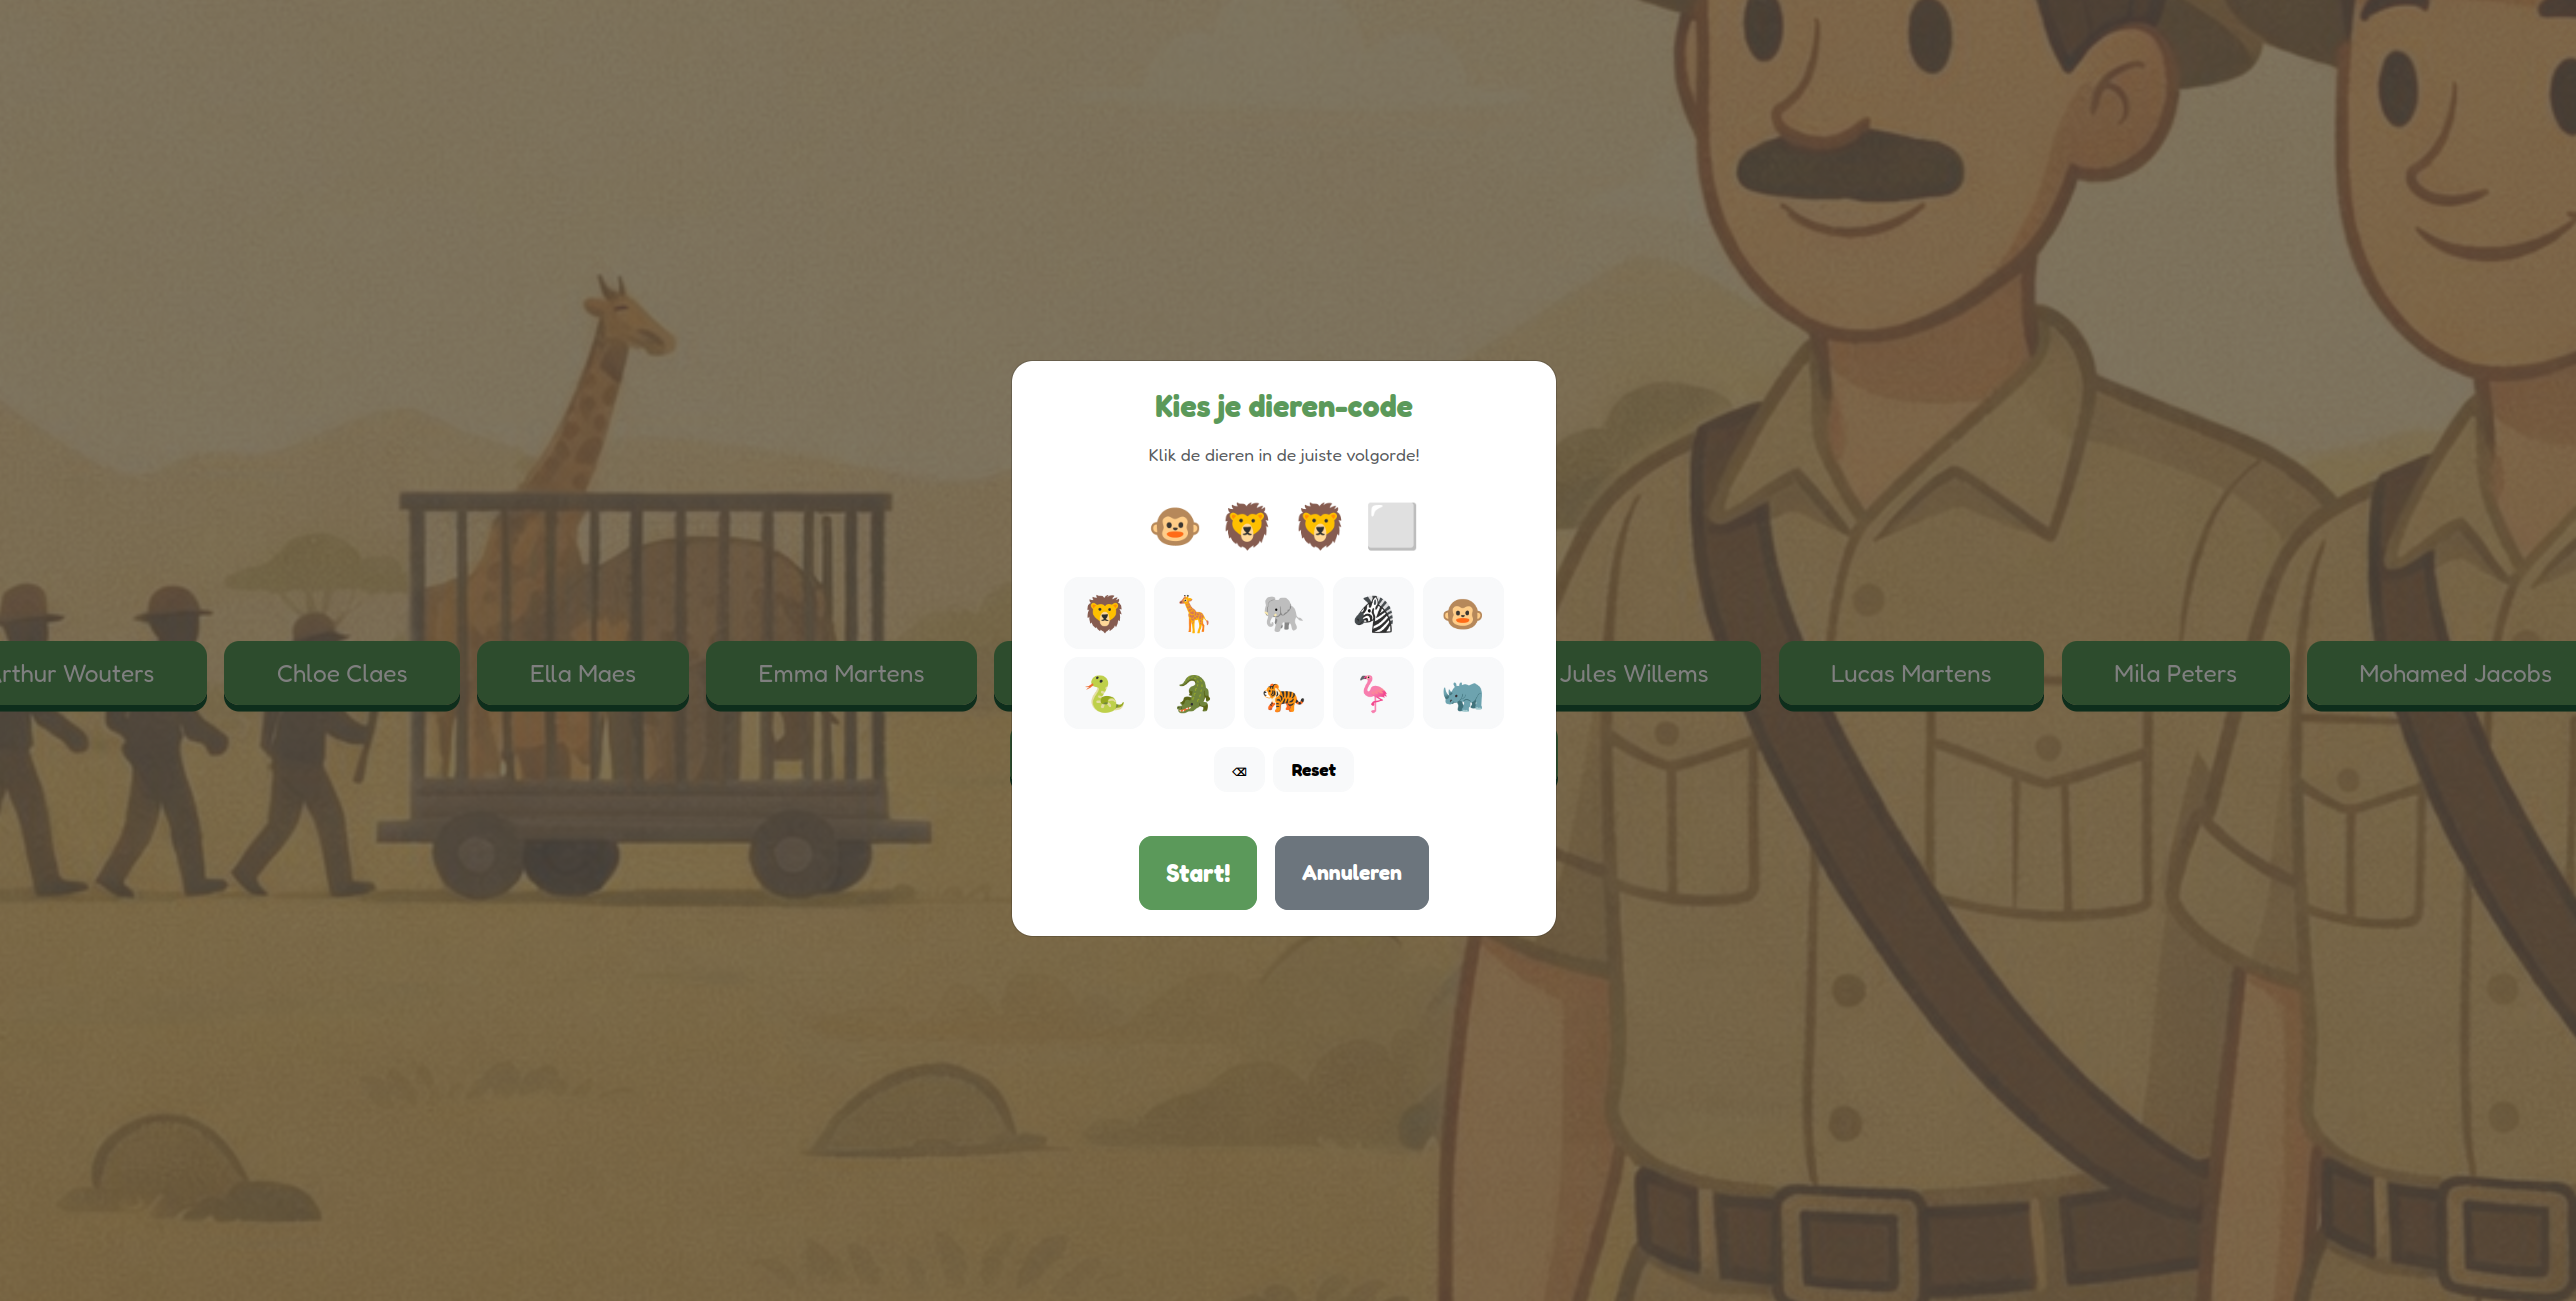
\includegraphics[width=0.8\textwidth]{figures/animal-login.png}
        \caption{The student login screen. After selecting their name, the child enters their personal animal code by clicking four animal icons in the correct order.}
        \label{fig:animal-login}
    \end{subfigure}
    \hfill
    \begin{subfigure}[t]{\textwidth}
         \vspace{0.5cm} 
        \centering
        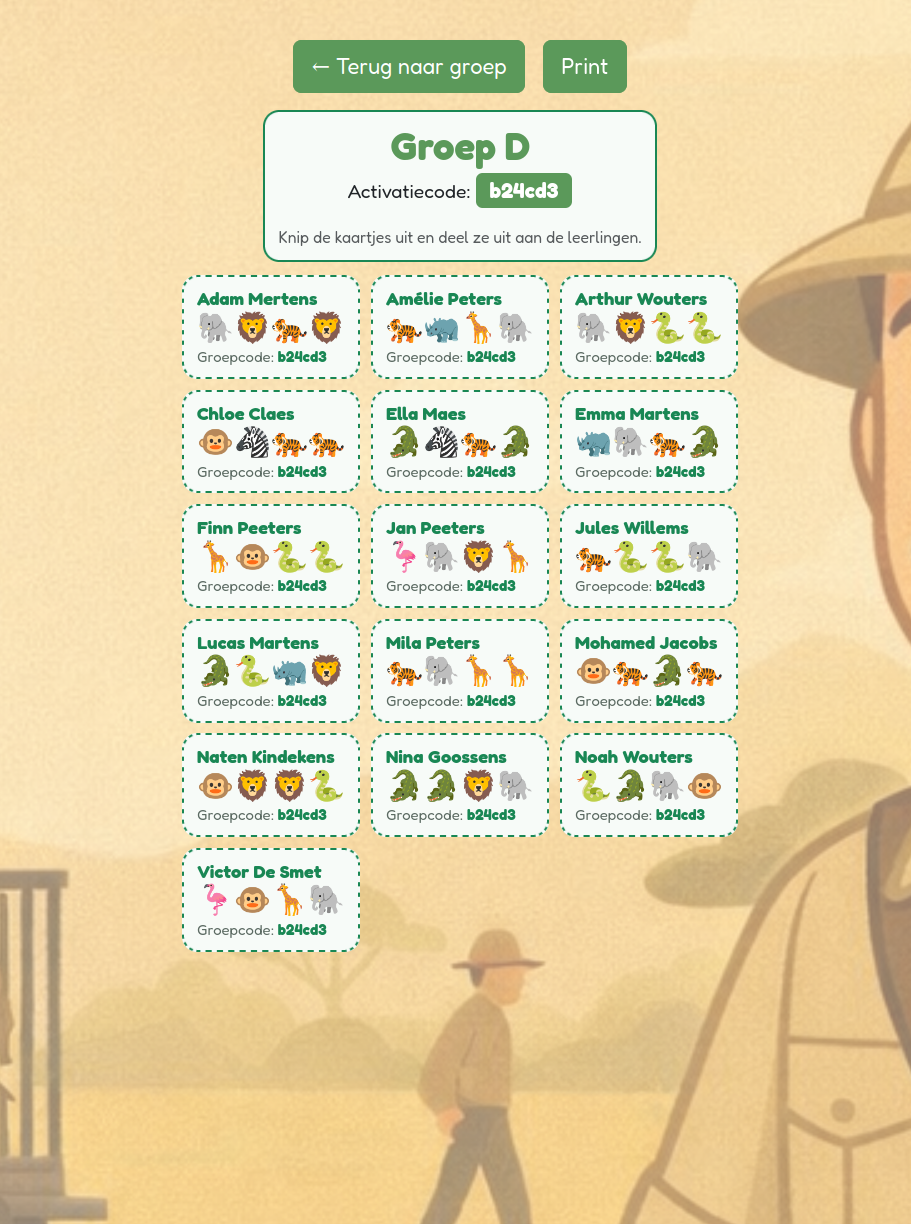
\includegraphics[width=0.4\textwidth]{figures/login-cards.png}
        \caption{Printable login cards generated through the teacher dashboard. Each card shows the child's name, group code, and personal animal code, and can be taken home for use outside the classroom.}
        \label{fig:login-cards}
    \end{subfigure}
    \caption{The RekenRangers login system. Children access the platform using a group code and a personal animal code, both provided through printable cards distributed by the teacher or researcher.}
    \label{fig:accessibility}
\end{figure}

Teachers and researchers generate these cards through the group management screen in the teacher dashboard. The cards can be printed and handed out in class, and since they contain everything a child needs to log in, they also enable use at home. This low-threshold approach to access means that RekenRangers can serve as both a classroom tool and a home practice tool without any additional setup.

\subsection{User friendliness}
The final exercise-tool property is user friendliness, and for RekenRangers this is less a single feature than a principle that runs through every screen of the application. The target audience is children between seven and eleven years old, and every interface element was designed with that in mind. Buttons are large and clearly labelled, navigation follows a simple top-to-bottom flow, and the visual language uses colours, icons, and illustrations rather than relying on text. All text that does appear is written in simple, child-appropriate Dutch.

To help children get started without needing an adult to explain the tool, RekenRangers includes an interactive demo mode. The demo walks the child through the full exercise flow step by step: how to read and answer an exercise, how to submit their answer, how the coin reward works, and how to navigate to the puzzle screen. When the metacognitive self-assessment setting is enabled, a separate version of the demo is available that also explains the smiley-based confidence judgement and what the feedback on it means. The demo can be replayed at any time, so a child who is unsure about something mid-session can revisit the explanation without having to ask for help.

One specific design decision worth mentioning is that the entire child-facing interface can be operated using only the keyboard. Answers are typed in directly, smileys are selected with the f,g,h,j keys, and puzzle pieces are bought with the spacebar. This was a deliberate choice. In pilot sessions, we observed that mouse and trackpad interactions introduced variability in response times that had nothing to do with arithmetic ability. By making the keyboard the primary input method, the tool removes a source of noise from the data, which matters both for the child's experience and for the quality of the research data collected.

The goal behind all of these choices is the same one that Section \ref{sec:exercise-properties} identified through cognitive load theory \cite{sweller1988cognitive}: the interface should be invisible. Every moment a child spends figuring out where to click or what a button means is a moment they are not spending on arithmetic. A well-designed exercise tool is one where the child forgets they are using a tool at all.